\documentclass[tikz,border=2pt]{standalone}
\usepackage{amsmath,amssymb}
\usepackage{tikz}

\begin{document}
% Mult(3, (1/2, 1/4, 1/4)): the ten possible count vectors (n1, n2, n3) with n1+n2+n3 = 3 on a
% triangular lattice; disc area is proportional to the probability.
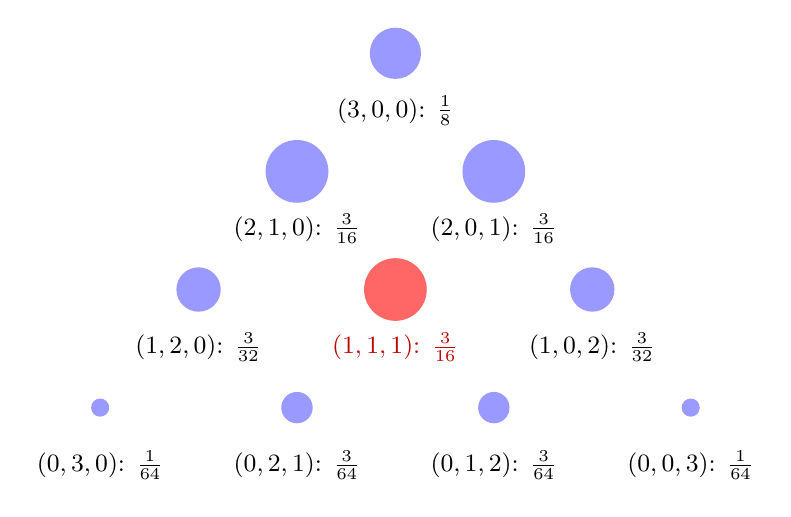
\begin{tikzpicture}[every node/.style={font=\small}]
	\foreach \a/\b/\c/\p/\lab in {3/0/0/8/{\tfrac18}, 2/1/0/12/{\tfrac3{16}}, 2/0/1/12/{\tfrac3{16}}, 1/2/0/6/{\tfrac3{32}}, 1/0/2/6/{\tfrac3{32}}, 0/3/0/1/{\tfrac1{64}}, 0/2/1/3/{\tfrac3{64}}, 0/1/2/3/{\tfrac3{64}}, 0/0/3/1/{\tfrac1{64}}} {
		\pgfmathsetmacro{\px}{(\c-\b)*1.25}
		\pgfmathsetmacro{\py}{\a*1.5}
		\pgfmathsetmacro{\r}{0.115*sqrt(\p)}
		\fill[blue!40] (\px,\py) circle (\r);
		\node[anchor=north] at (\px,\py-0.42) {$(\a,\b,\c)$: $\lab$};
	}
	\fill[red!60] (0,1.5) circle (0.398);
	\node[anchor=north, red!75!black] at (0,1.08) {$(1,1,1)$: $\tfrac3{16}$};
\end{tikzpicture}
\end{document}
